\section{Grundlagen} 
\subsection{Adversarial Attacks}

Adversarial Attacks sind ein faszinierendes Phänomen im Bereich des Deep Learning, das in den letzten Jahren zunehmend an Bedeutung gewonnen hat. Bei diesen Angriffen auf Bildklassifikationsmodelle werden die Eingabewerte durch eine minimale Veränderung modifiziert, die vom menschlichen Auge nicht mehr wahrnehmbar ist. Diese Angriffe beziehen sich auf gezielte Manipulationen von Eingabedaten, die darauf abzielen, neuronale Netzwerke zu täuschen und falsche Vorhersagen zu erzwingen. Sie werfen wichtige Fragen zur Robustheit und Sicherheit von Deep Learning Modellen auf und haben weitreichende Implikationen für deren praktische Anwendungen \cite{goodfellow_explaining_2015}. 

\subsubsection{Adversarial Attacks Schema} 

Die Abbildung \ref{fig:grundlagen} illustriert den allgemeinen adversarial Attacke auf ein beliebiges Model $c$. 

\begin{figure}[H]
    \centering
    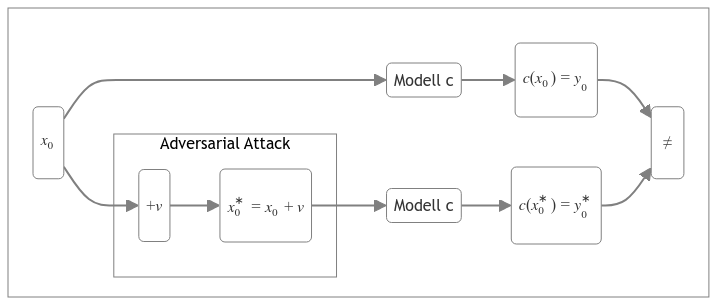
\includegraphics[width=13.5cm]{01-images/02-grundlagen/adversarial-attack.png}
    \caption{Vorgang einer Attacke}
    \label{fig:grundlagen}
\end{figure}

\begin{itemize}
    \item $x_0$, ist der Eingabewert, dies kann ein Signal, Bild oder sonstige Formate sein.
    \item $v$, ist die Perturbation, die Störung.
    \item $x_0^{*}$, der veränderte, attackierte Eingabewert durch die Perturbation.
    \item $c$, Das Modell, welche die Eingabe verarbeitet und Output generiert.
    \item $y_0$, Output des Modells durch den unveränderten Eingabewert.
    \item $y_0^{*}$, Output des Modells durch den attackierte Eingabewert.
    \item $\neq$, der Output von $y_0$ und $y_0^{*}$ ist nicht gleich.
\end{itemize}


\subsubsection{Beispiele für Adversarial Attacks} 

\todo{one pixel attack}

Ein faszinierendes Beispiel für physische Adversarial Attacks ist das  ``Adversarial T-Shirt'', das in der Lage ist, Personenerkennungssysteme zu täuschen \cite{xu_adversarial_2020}. Dieses T-Shirt ist mit speziellen Mustern bedruckt, die darauf ausgelegt sind, die Algorithmen von Objekterkennungssystemen zu täuschen. Im Gegensatz zu herkömmlichen Angriffen, die oft statische Objekte wie Stopp Schilder oder Gesichtserkennung nutzen, bezieht sich dieses Beispiel auf ein dynamisches Objekt – ein T-Shirt auf einem bewegenden Menschen \cite{xu_adversarial_2020}. 

Der ``One Pixel Attack'' \cite{su_one_2019} ist eine Technik, die darauf abzielt, Deep Neural Networks durch die Modifikation nur eines einzigen Pixels in einem Bild zu täuschen. Diese Methode offenbart die hohe Sensitivität von \acrlong{dnn}s gegenüber minimalen Veränderungen in den Eingabedaten. Basierend auf einer ``differential evolution'' Strategie, wird der effektivsten Pixel sowie dessen Farbänderung ermittelt, um eine Fehlklassifizierung durch das Netzwerk zu erzeugen. Trotz der geringfügigen Bildmodifikation, ist diese Attacke in der Lage, die Klassifizierungssicherheit von \acrlong{dnn}s signifikant zu beeinträchtigen.
In Experimenten mit dem CIFAR-10 Datensatz konnte durch die Veränderung eines einzelnen Pixels in einem Bild, das ursprünglich korrekt als ``Automobil'' klassifiziert wurde, eine Fehlklassifizierung als ``Vogel`` mit einer Erfolgsrate von etwa 70\% erzielt werden. Die spezifische Auswahl des Pixels und dessen Farbe wird durch den Optimierungsalgorithmus bestimmt, der darauf ausgerichtet ist, die Wahrscheinlichkeit einer Fehlklassifizierung zu maximieren .

\subsection{Universal Adversarial Attacks auf Bildklassifikation} 

Bei der Universal Adversarial Attacks wird eine "Universelle" Perturbation erzeugt, welches mehrere Modelle und unabhängig vom Datensatz auf alle Bilder addiert werden kann und das Modell somit zu einer Fehlklassifikation geschieht. 

\subsubsection{Grundlagen}

Adversarial Attacks nutzen Schwachstellen in den Entscheidungsgrenzen von Klassifizierungsmodellen aus, indem sie gezielt minimale, aber effektive Veränderungen an den Eingabedaten vornehmen. Diese Veränderungen, oft als Perturbation bezeichnet, sind typischerweise für das menschliche Auge kaum wahrnehmbar, können jedoch das Modell dazu bringen, eine falsche Vorhersage zu treffen. Ein wesentliches Merkmal der universalen Perturbation ist ihre Übertragbarkeit über verschiedene Modelle und Daten hinweg, was sie besonders bedrohlich in realen Anwendungen macht.

\subsubsection{Unser Hauptpaper}

Unser Hauptpaper ``Universal adversarial perturbations'' von Moosavi-Dezfooli et al. (2017) \cite{moosavi-dezfooli_universal_2017} bildet die Grundlage dieser Bachelorarbeit. Die Autoren demonstrieren die Existenz von universellen Perturbationen, die die Fähigkeit besitzen, mit hoher Wahrscheinlichkeit fehlerhafte Klassifizierungen über verschiedene Modelle und Datensätze hinweg zu induzieren. Ihre Forschung unterstreicht die signifikanten Sicherheitsrisiken, die durch solche Angriffe entstehen können, und betont die Notwendigkeit robusterer Verteidigungsmechanismen gegenüber adversarial attacks.

\subsubsection{Bisherige Herausforderungen bei der Verteidigung}

\todo{verteidigung}

\subsection{Anwendungsfall}

Angesichts der Vielfalt an möglichen Konfigurationen für die Generierung der Attacken und der Robustifizierung der Modelle, basieren unsere Entscheidungen bezüglich der Parameterwahl auf einem speziell ausgewählten Anwendungsfall. 
\\
\\
In dieser Arbeit liegt der Schwerpunkt auf der Anwendung von Universal Adversarial Attacks auf Systeme zur Erkennung kritischer Krankheiten. Ein besonderes Augenmerk wird darauf gelegt, dass schon eine Täuschungsrate von nur 20\% bei positiv klassifizierten Bildern, die fälschlicherweise als negativ eingestuft werden, eine erhebliche Sicherheitslücke darstellen kann. Derartige Fehlklassifikationen in medizinischen Diagnosesystemen können gravierende Folgen haben, da sie potenziell zu einer Unterbehandlung von kritischen Gesundheitszuständen führen. Die Herausforderung besteht darin, die Perturbationen so zu gestalten, dass sie minimal und für das menschliche Auge schwer erkennbar sind, um nicht nur die Unsichtbarkeit der Manipulationen zu gewährleisten. Diese Anforderung ist entscheidend, da eine offensichtliche Verzerrung des Bildes im medizinischen Kontext sofort Misstrauen erwecken und somit schnell identifiziert werden könnte. Durch die subtile Anwendung der Perturbationen streben wir an, die Balance zwischen Effektivität der Angriffe und deren Unauffälligkeit zu optimieren. Die Ergebnisse dieser Arbeit könnten für die Entwicklung von sichereren, Adversarial robusten medizinischen Diagnosesystemen haben.